\section{我的老腰受不了了——如何保持颈椎、腰椎健康}

\begin{newminipage}[0.39]
    \begin{figure}[H]
        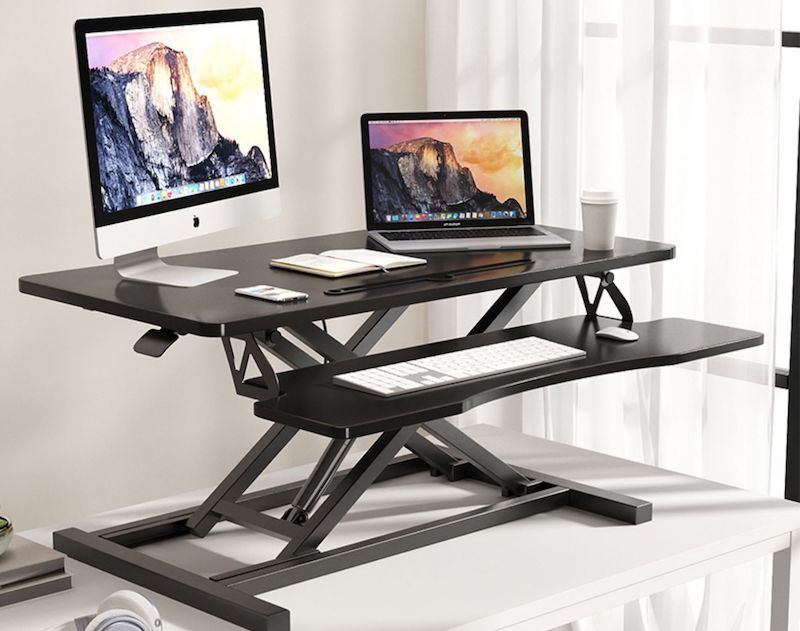
\includegraphics[width=0.95\columnwidth, right]{author-folder/Yue.Zhou/gongzuotai.jpg}
    \end{figure}
\end{newminipage}
\begin{newminipage}[0.6]
    在没有读博之前,我就患上了严重的腰肌劳损。这个玩意怎么说呢,说是大病吧,他不是,但无时无刻不在折磨着你。最严重的时候,疼的我晚上都睡不着。去医院看过也开过药,但医生说这个病需要自己保养,无法根治。后来我试着跑了半年步,哎!腰肌劳损神奇的好了,现在一点都不疼了(如遇久坐,仍旧是不行的,会疼)。读博之后也没有心情运动了,于是买了一个升降工作台(推荐人手一个!太好用了!)。可以站着办公,站累了就坐下办公。极大程度上杜绝了久坐对腰椎的伤害。
\end{newminipage}


\begin{flushright}
(2022年12月30日 by Yue Zhou)
\end{flushright}


